\documentclass[beamer]{standalone}

\usetheme{naked}
\setbeamercolor{alerted text}{fg=green!50!black}
\setbeamercolor{box title}{fg=purple}
\setbeamertemplate{frametitle}{}

% \usepackage{xkeyval}
% \usepackage{pgffor}

\usepackage{standalone}

\makeatletter
../code-graphs.tex
\makeatother

% vertical centering of cells
% see http://tex.stackexchange.com/questions/46386/vertically-center-cells-of-a-table
\usepackage{array}% http://ctan.org/pkg/array
\newcolumntype{M}{>{\centering\arraybackslash}m{\dimexpr.17\linewidth-2\tabcolsep}}

% remove space between margin and lists
\usepackage{enumitem}
\setitemize{label=\usebeamerfont*{itemize item}%
  \usebeamercolor[fg]{itemize item}
  \usebeamertemplate{itemize item}}
\setlist{leftmargin=*,labelindent=0cm}

%\usepackage{amsmath}

\usepackage{tikz}
\usepackage{tkz-graph}
\usepackage{tkz-berge}
\usepackage{tkz-berge-add}

\usepackage[utf8]{inputenc}
% \usepackage{libertine}
% \usepackage[libertine]{newtxmath}

%\usepackage{lxfonts}

\usepackage{cabin}
\usepackage{mathastext}

\newcommand{\graphcaption}[4][gray!80!white]{\draw (#2,#3) node [fill=#1]{#4};}

\SetVertexSimple[FillColor=gray, MinSize=10pt, LineWidth=1.5pt]

\tikzset{EdgeStyle/.style= {%
    color           = white,
    double          = black,
    double distance = 2.5pt}}

\newcommand{\setof}[2]{\left\{\,#1\mid #2\,\right\}}

\newcommand{\triangulo}[4]{%
  \shadedraw[inner color=#4,opacity=0.8,line width=1pt]
  (#1.center) -- (#2.center) -- (#3.center) -- cycle;}

\newcommand{\triangleshaded}[3]{%
  \draw[fill=gray]
  (#1.center) -- (#2.center) -- (#3.center) -- cycle;}

\newcommand{\triang}[3]{%
  \shadedraw[inner color=gray,,opacity=0.8,line width=1pt]
  (#1.center) -- (#2.center) -- (#3.center) -- cycle;}

\begin{document}

\begin{standaloneframe}

  \vspace{\fill}
  
  \uncover<1->{%
    \begin{minipage}{0.6\linewidth}
      Un \alert{morfismo de gráficas} $f\colon G\to L$ es una función
      tal que $x\sim y$ implica $f(x)\sim f(y)$ o $f(x)=f(y)$.
    \end{minipage}}%
  \uncover<2->{%
    \begin{minipage}{0.4\linewidth}
      \centering
      \begin{tikzpicture}
        \grMan[RA=0.8]
        \AddVertexColor{red}{a0,a1,a2,a3}
        \AddVertexColor{blue}{a4,a5,a6}
        \AddVertexColor{green}{a7}
        \AddVertexColor{orange}{a8,a9}
      \end{tikzpicture}
      \hspace{0.5cm}
      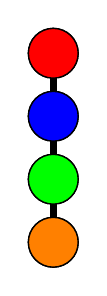
\begin{tikzpicture}
        \grPath[form=2,rotation=90,RA=0.8]{4}
        \AddVertexColor{red}{a3}
        \AddVertexColor{blue}{a2}
        \AddVertexColor{green}{a1}
        \AddVertexColor{orange}{a0}
      \end{tikzpicture}
    \end{minipage}}

  \vspace{\fill}

  \uncover<3->{%
    \begin{minipage}{0.6\linewidth}
      Si $L$ es una subgráfica de $G$, una \alert{retracción} $r\colon
      G\to L$ es un morfismo tal que $r(x)=x$ para todo $x\in L$.
    \end{minipage}}%
  \uncover<4->{%
    \begin{minipage}{0.4\linewidth}
      \centering
  \begin{center}
    \setxyzvec[17]
    \begin{tikzpicture}[scale=0.5]%
      [x = {(\xone cm,\yone cm)}, y = {(\xtwo cm,\ytwo cm)}, z =
      {(0cm,1cm)}]
      \begin{scope}[canvas is xy plane at z=0]
        \grEmptyCycle[RA=2,prefix=a,rotation=35]{4}
      \end{scope}
      \begin{scope}[canvas is xy plane at z=-2.5]
        \Vertex{x}
      \end{scope}
      \begin{scope}[canvas is xy plane at z=2.5]
        \Vertex{y}
      \end{scope}
      \EdgeFromOneToAll{x}{a}{}{4}
      \EdgeInGraphLoop{a}{4}
      \EdgeFromOneToAll{y}{a}{}{4}
      \uncover<1>{\graphcaption{6}{6}{$O_{3}$}}
      \uncover<2->{%
        \begin{scope}[canvas is xy plane at z=2.5]
          \Vertex[x=2,y=-2]{z}
        \end{scope}
        \EdgeFromOneToSel{z}{a}{}{0,3} \Edge(z)(y)
      }
      \uncover<3->{%
        \begin{scope}[canvas is xy plane at z=-2.5]
          \Vertex[x=2,y=-2]{w}
        \end{scope}
        \EdgeFromOneToSel{w}{a}{}{0,3} \Edge(w)(x)
      }
      \uncover<4->{\Edge(z)(w)}
      \uncover<5>{%
        {\SetUpEdge[color=magenta,lw=3pt]
          \Edge[style={bend right=45,->}](z)(a3)
          \Edge[style={bend right=45,->}](w)(a0)}
        \graphcaption[magenta]{7}{7}{retracción}
      }
    \end{tikzpicture}
  \end{center}
    \end{minipage}}

  \vspace{\fill}

\end{standaloneframe}

\end{document}
